This chapter provides an overview of the Single Chip Mote digital system software and software development tools. While the majority of the work on the Single Chip Mote is focused on hardware design, the overall goal of this project is to work in collaboration with software developers to design a platform ideal for Internet of Things (IoT) applications. In particular, the Single Chip Mote team is collaborating with the developers of OpenWSN \cite{openwsn}, an open-source protocol stack designed for IoT. With their advanced embedded systems experience, the developers of OpenWSN can provide feedback for hardware improvements while they port OpenWSN onto the Single Chip Mote. Through the use of FPGAs, hardware changes can quickly be verified, fine-tuned, and integrated into the software. The information in this chapter contains the basics for writing software that uses the digital system peripherals in order to facilitate application development.

\section{Keil Project Settings} \label{keil-project-settings}
Keil projects have already been created for the main software running on the Cortex-M0 and the basic firmware (chapter \ref{bootloading}) used to load the main software onto the Single Chip Mote digital system. However, it may be necessary in the future to create new projects for different applications or variations of the Single Chip Mote hardware. This section contains the information needed to create a new project in Keil uVision 5 for the ARM Cortex-M0 on the Single Chip Mote digital system.

\subsection{New Project and Device Selection}
To create a new project, open Keil uVision 5 and select the New uVision Project... option in the Project menu. This will bring up the Device Selection, displaying all of the ARM cores supported by the IDE. The device for the Single Chip Mote digital system is found under ARM > ARM Cortex M0 > ARMCM0, as shown in Figure \ref{fig:keil-cpu-selection}. Select ARMCM0 and then select Next.

The Manage Runtime Environment window in Figure \ref{fig:keil-manage-runtime-environment} displays options for including additional software drivers from ARM. The default settings are sufficient for the Single Chip Mote. Select OK to finish creating the project.

\begin{figure}
\centering
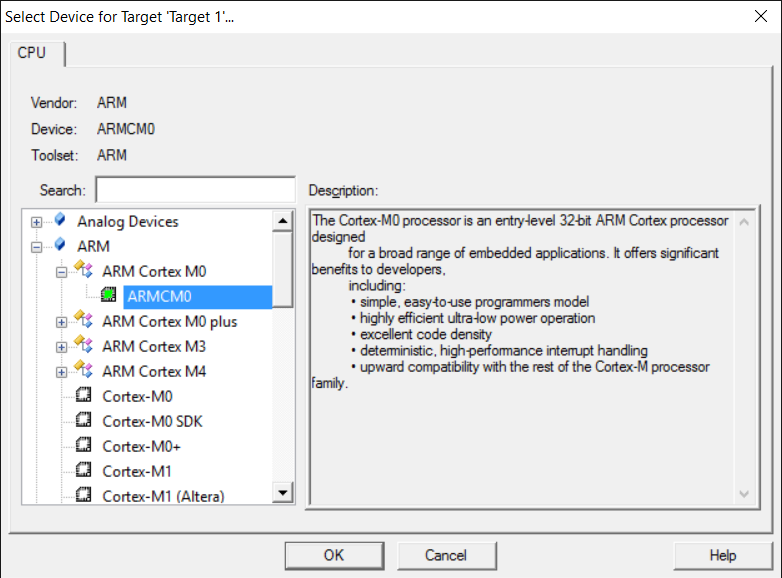
\includegraphics[width=0.7\linewidth]{keil-cpu-selection}
\caption{Device selection window in Keil}
\label{fig:keil-cpu-selection}
\end{figure}

\begin{figure}
\centering
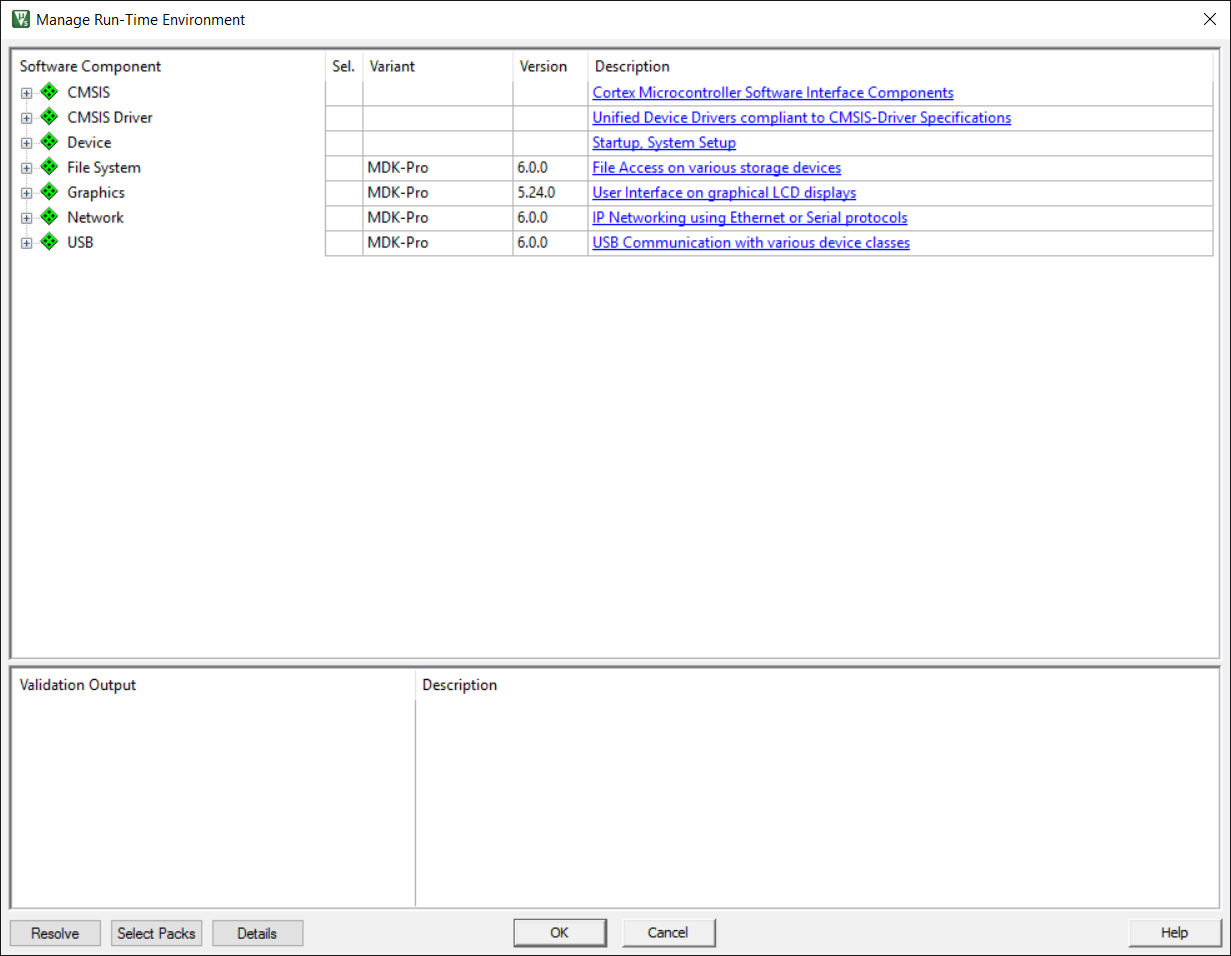
\includegraphics[width=0.7\linewidth]{keil-manage-runtime-environment}
\caption{Manage Runtime Environment window in Keil}
\label{fig:keil-manage-runtime-environment}
\end{figure}

\subsection{Target Options}
The Target Options window contains the settings that describe the memory resources on the device, the compiler and linker options, and the debug options. To access the Target Options window, right-click Target 1 in the Project panel, and select Options for Target `Target 1' (see Figure \ref{fig:keil-options-for-target}).

The Target Options window has 10 tabs:

\begin{description}
	\item[Device] This tab is used to select or change the CPU for the project. This is similar to the Device Selection window in Figure \ref{fig:keil-cpu-selection}.
	\item[Target] This tab, shown in Figure \ref{fig:keil-target-options}, specifies the CPU clock frequency (in the box labeled Xtal (MHz)), operating system, and memory regions. For the Single Chip Mote digital system, the frequency is 5MHz, and there is no operating system. There is one read-only memory area, corresponding to the instruction memory, and one read-write memory, corresponding to the data memory. The instruction memory is specified as on-chip memory with a start address of \texttt{0x0}. The size field indicates the size of the memory in bytes, where 64kB is represented in hex as \texttt{0x10000}. The startup option indicates that the code is loaded from this memory on startup. The data memory is specified as on-chip memory with a start address of \texttt{0x20000000}. The size is also 64kB (represented in hex as \texttt{0x10000}).
	\item[Output] This tab, shown in Figure \ref{fig:keil-output-options}, specifies the name of the build output (in the box labeled Name of Executable), and the type of output (executable or library). The Single Chip Mote requires an executable, and the output is called \url{code.axf}. The check boxes labeled Debug Information, Create HEX File, Browse Information, and Create Batch File are not required for the Single Chip Mote.
	\item[Listing] This tab contains compiler and linker options. The default settings for this tab are sufficient.
	\item[User] This tab, shown in Figure \ref{fig:keil-user-options}, provides the option to run programs before compilation or before/after builds. For the Single Chip Mote, one program must be run after the build to convert \path{code.axf} to a binary file, \path{code.bin}. This is done by running the following command: \texttt{fromelf --bin code.axf -o code.bin}. Another program can optionally be run to convert \path{code.axf} to a disassembled text file. The disassembled file lists the assembly code in \path{code.axf} in a human-readable form, and may be useful for debugging purposes. This is done by running the following command: \texttt{fromelf -cvf code.axf -o disasm.txt}.
	\item[C/C++] This tab contains additional compiler options. The default settings for this tab are sufficient.
	\item[Asm] This tab contains the assembler options. It is recommended that the Thumb Mode option is checked for the Single Chip Mote. Thumb Mode uses 16-bit instructions instead of 32-bit instructions when possible, with the overall effect of reduced code size.
	\item[Linker] This tab, shown in Figure \ref{fig:keil-linker-options}, contains additional linker options. It is recommended that the Use Memory Layout from Target Dialog box is checked. This means that the memory regions defined in the Target tab are used to generate a scatter file (called \path{code.sct}) that describes the available memory regions for the linker. If this box is unchecked, then a scatter file must be provided in the Scatter File box.
	\item[Debug] This tab contains the debug options. Since the ARM Cortex-M0 DesignStart processor does not have debug capabilities, the settings in this tab make no difference.
	\item[Utilities] This tab contains the options for flashing the software onto a device using Keil. This is currently not possible with the Single Chip Mote, and therefore the settings in this tab make no difference.
\end{description}

Overall, the default settings in the Target Options window are sufficient for basic applications on the Single Chip Mote. Further fine-tuning and customization is recommended in the future for more optimized code generation.

\begin{figure}
\centering
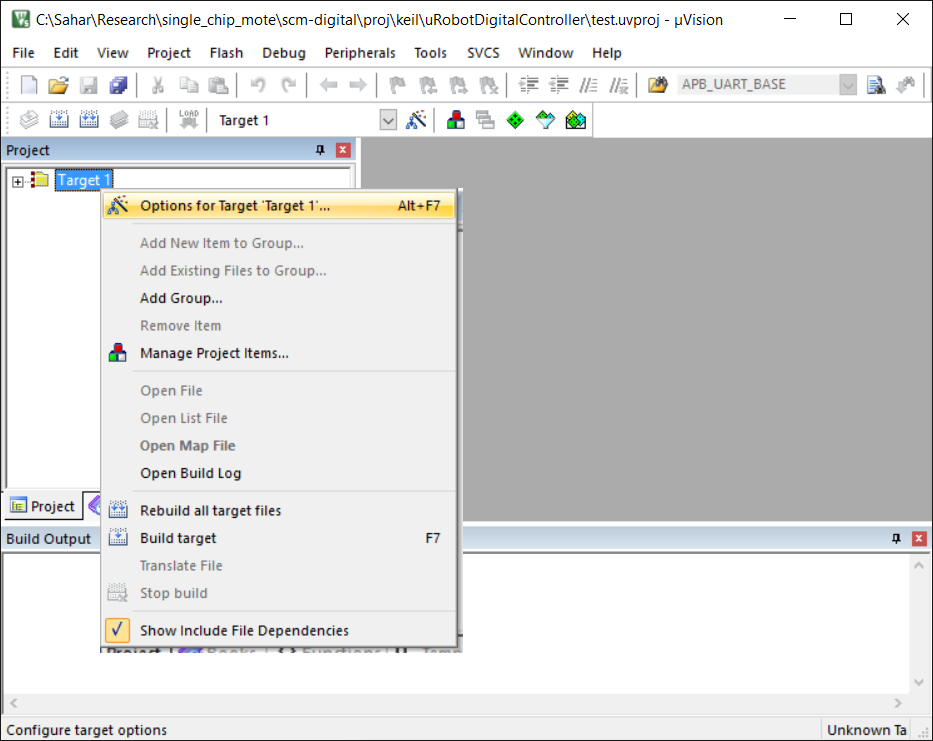
\includegraphics[width=1\linewidth]{images/keil-options-for-target}
\caption{Opening the Target Options window}
\label{fig:keil-options-for-target}
\end{figure}

\begin{figure}
\centering
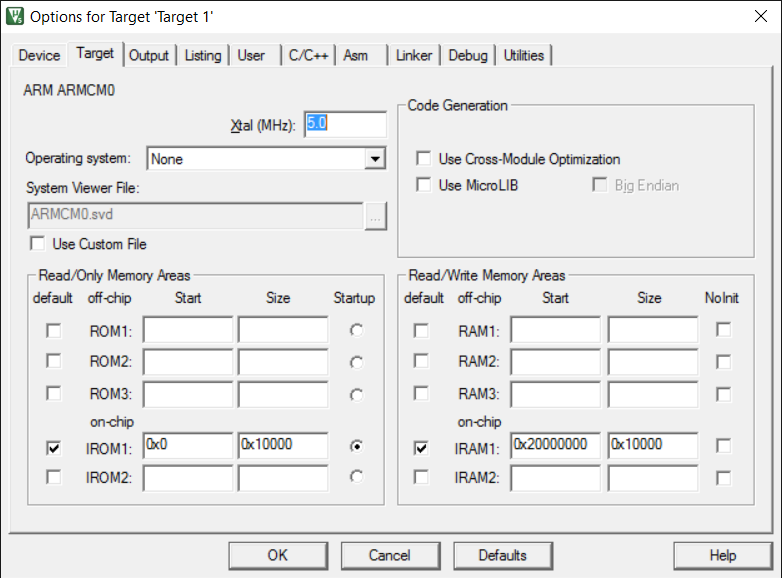
\includegraphics[width=0.9\linewidth]{keil-target-options}
\caption{Target tab in the Target Options window}
\label{fig:keil-target-options}
\end{figure}

\begin{figure}
\centering
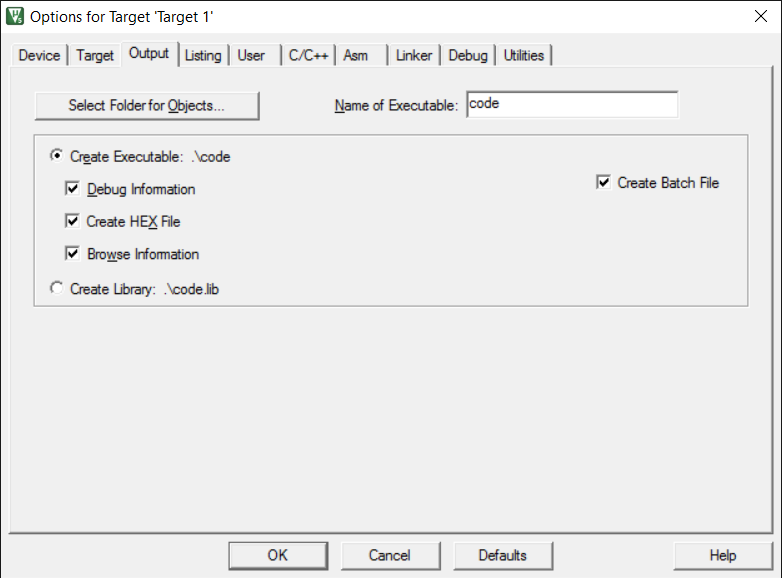
\includegraphics[width=0.9\linewidth]{keil-output-options}
\caption{Output tab in the Target Options window}
\label{fig:keil-output-options}
\end{figure}

\begin{figure}
\centering
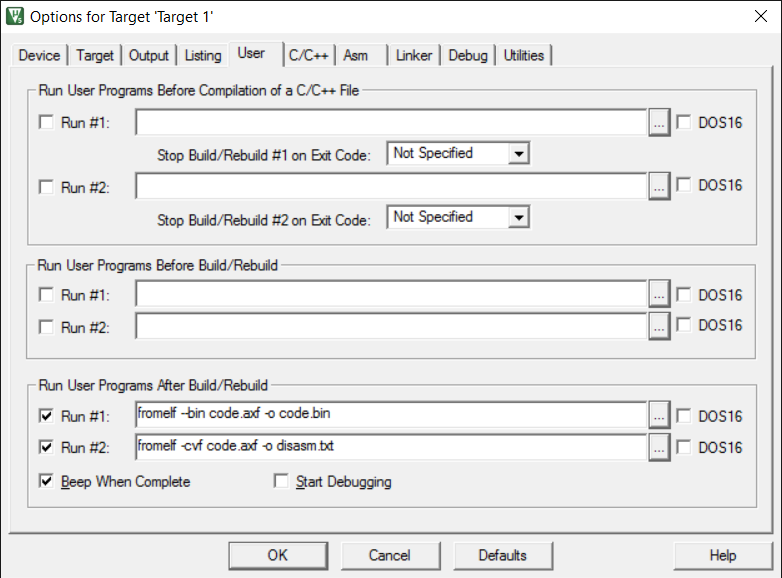
\includegraphics[width=0.9\linewidth]{keil-user-options}
\caption{User tab in the Target Options window}
\label{fig:keil-user-options}
\end{figure}

\begin{figure}
\centering
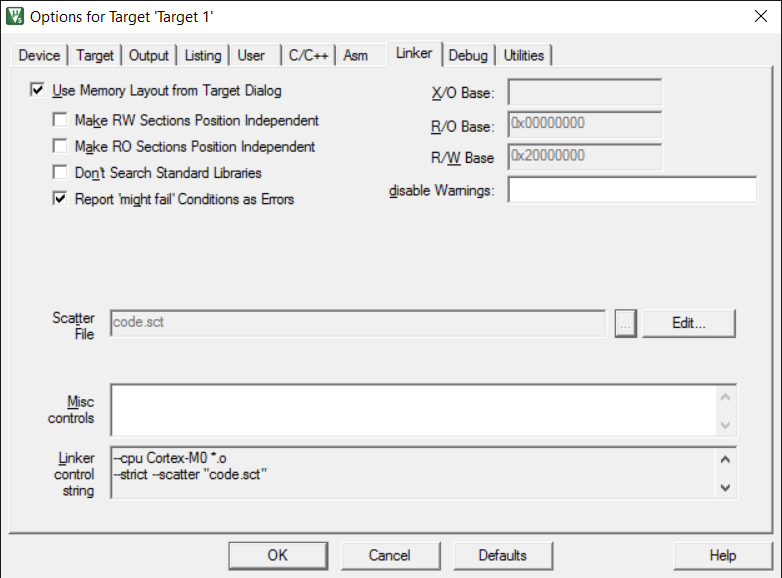
\includegraphics[width=0.9\linewidth]{keil-linker-options}
\caption{Linker tab in the Target Options window}
\label{fig:keil-linker-options}
\end{figure}

\subsection{Scatter File Settings}
A scatter file describes the memory regions available to a microcontroller for the linker. Keil can generate a scatter file based on settings provided in the Target Options window. Below is an example of the scatter file automatically generated by Keil for the Single Chip Mote. For more information on scatter file see Chapter 4 of the ARM compiler toolchain Version 5.0 Linker Reference \cite{linker-reference}.

\begin{lstlisting}
; *************************************************************
; *** Scatter-Loading Description File generated by uVision ***
; *************************************************************

LR_IROM1 0x00000000 0x00010000  {    ; load region size_region
    ER_IROM1 0x00000000 0x00010000  {  ; load address = execution address
        *.o (RESET, +First)
        *(InRoot$$Sections)
        .ANY (+RO)
    }
    RW_IRAM1 0x20000000 0x00010000  {  ; RW data
        .ANY (+RW +ZI)0.9
    }
}
\end{lstlisting}

\section{Required Assembly, Header, and C Files}
The Cortex-M0 DesignStart processor on the Single Chip Mote digital system is programmed using a combination of C, C++, and ARM assembly code in Keil. Each project in Keil requires some basic assembly code for initial startup (found in \texttt{cm0dsasm.s}), a C header file with the addresses of the memory-mapped registers on the Single Chip Mote (found in \texttt{Memory\_Map.h}), a file with C code to implement \texttt{printf} over UART (found in \texttt{retarget.c}), and finally any files with the \texttt{main} function and any other code required for the application.

\subsection{cm0dsasm.s}
This file is based on an example provided in the ARM Cortex-M0 DesignStart kit. This file contains ARM assembly code required by the Cortex-M0 in order to handle startup, resets, and interrupts properly.

The first section of this code (shown below) defines the size and properties of the stack and heap. The size of the stack and heap must add up to be less than or equal to the available data memory. Note that not all data is stored on the stack or heap; global variables are stored in a special section of memory. If the program has any global variables, the size of the stack and heap must be less than the data memory in order to leave room for those variables.

\begin{lstlisting}
Stack_Size      EQU     0x0800                          ; 4KB of STACK

                AREA    STACK, NOINIT, READWRITE, ALIGN=4
Stack_Mem       SPACE   Stack_Size
__initial_sp	


Heap_Size       EQU     0x0400                          ; 2KB of HEAP

                AREA    HEAP, NOINIT, READWRITE, ALIGN=4
__heap_base				
Heap_Mem        SPACE   Heap_Size
__heap_limit
\end{lstlisting}

The second section of this code (shown below) defines the vector table. The vector table is a series of addresses defined at the beginning of a program that point to reset handlers, exception handlers, and interrupt handlers. Each line beginning with \texttt{DCD} initializes one word of memory with the value written after \texttt{DCD}:

\begin{lstlisting}
; Vector Table Mapped to Address 0 at Reset

                    PRESERVE8
                    THUMB

                        AREA    RESET, DATA, READONLY
                        EXPORT  __Vectors

__Vectors               DCD     __initial_sp
                        DCD     Reset_Handler
                        DCD     0
                        DCD     0
                        DCD     0
                        DCD     0
                        DCD     0
                        DCD     0
                        DCD     0
                        DCD     0
                        DCD     0
                        DCD     0
                        DCD     0
                        DCD     0
                        DCD     0
                        DCD     0

; External Interrupts

                        DCD     UART_Handler
                        DCD     0
                        DCD     0
                        DCD     ADC_Handler
                        DCD     0
                        DCD     0
                        DCD     RF_Handler
                        DCD     RFTIMER_Handler
                        DCD     0
                        DCD     0
                        DCD     0
                        DCD     0
                        DCD     0
                        DCD     0
                        DCD     0
                        DCD     0
\end{lstlisting}

The first 16 entries in the vector table (and their addresses in the vector table) are: initial stack pointer value (\texttt{0x00}), Reset handler address (\texttt{0x04}), NonMaskable Interrupt handler address (\texttt{0x08}), HardFault handler address (\texttt{0x0C}), Reserved (\texttt{0x10-0x28}), SVCall (\texttt{0x2C}), Reserved (\texttt{0x30-0x34}), PendSV (\texttt{0x38}), and SysTick (\texttt{0x3C}). If one of the exception handlers is not implemented, then the address is specified as 0. For more information, see the Cortex-M0 Devices Generic User Guide \cite{cortex-m0-generic-ug}.

The next 16 entries in the vector table are the addresses of the interrupt handlers for the 16 available external interrupts. In this case an external interrupt defines an interrupt generated outside of the Cortex-M0, including from peripherals on the Single Chip Mote. Each address in this section of the vector table corresponds to the one of the interrupt connections to the Cortex-M0 in the Single Chip Mote digital system. The following Verilog code defines a bus containing all of the interrupt connections to the Cortex-M0:

\begin{lstlisting}
assign IRQ = {8'b00000000,RFTIMER_IRQ,RF_IRQ,1'b0,1'b0,ADC_IRQ,1'b0,1'b0,UART_IRQ};
\end{lstlisting}

Note that unused interrupts are assigned to 0. Their corresponding address in the vector table are also zero. The \texttt{UART\_IRQ} signal, assigned to \texttt{IRQ[0]}, is connected to the \texttt{APBUART} module. The first address in the vector table corresponds to \texttt{IRQ[0]} and \texttt{UART\_IRQ}. The first address in the vector table is \texttt{UART\_Handler}, which is a label referring to a section of code in a later part of \texttt{cm0dsasm.s}.

The next section of code contains assembly code for the various exception and interrupt handlers found in the vector table. The reset handler enables the interrupts and then jumps to the \texttt{main} function defined in C code:

\begin{lstlisting}
Reset_Handler   PROC
        GLOBAL Reset_Handler
        ENTRY

        LDR     R1, =0xE000E100           ;Interrupt Set Enable Register
        LDR     R0, =0xFF                 ;<- REMEMBER TO ENABLE THE INTERRUPTS!!
        STR     R0, [R1]

        IMPORT  __main
        LDR     R0, =__main               
        BX      R0                        ;Branch to __main
                ENDP
\end{lstlisting}

The other interrupt handlers first mask other interrupts, call the interrupt handler written in C code, and unmask the interrupts
before returning:

\begin{lstlisting}
UART_Handler    PROC
        EXPORT UART_Handler
        IMPORT UART_ISR

        PUSH    {R0,LR}

        MOVS     R0, #1 ;         ;MASK all interrupts
        MSR PRIMASK, R0 ; 		

        BL UART_ISR


        MOVS    R0, #0         ;ENABLE all interrupts
        MSR PRIMASK, R0

        POP     {R0,PC}
                ENDP 
\end{lstlisting}

All interrupt handlers should follow this basic format. In the future it may be necessary to write additional exception handlers in assembly for unused exceptions such as the HardFault Interrupt or NonMaskable Interrupt.

The last part of this file initializes the stack and heap:

\begin{lstlisting}
; User Initial Stack & Heap
                IF      :DEF:__MICROLIB
                EXPORT  __initial_sp
                EXPORT  __heap_base
                EXPORT  __heap_limit
                ELSE
                IMPORT  __use_two_region_memory
                EXPORT  __user_initial_stackheap
__user_initial_stackheap

                LDR     R0, =  Heap_Mem
                LDR     R1, =(Stack_Mem + Stack_Size)
                LDR     R2, = (Heap_Mem +  Heap_Size)
                LDR     R3, = Stack_Mem
                BX      LR

                ALIGN

                ENDIF
\end{lstlisting}

\subsection{Memory\_Map.h}
This file is a C header file containing the addresses of the memory-mapped registers on the Single Chip Mote. The beginning of this file defines the base addresses of each peripheral. The addresses for each register are defined as an offset of the base address for the corresponding peripheral. The information in this file must match the information in the \texttt{REGISTERS.vh} Verilog header file found in \path{scm-digital/src/hw/artix-7/uRobotDigitalController/globalHeaders}. Note that each base address is defined as a hexadecimal number, whereas each register is defined as a dereferenced pointer to an unsigned integer:

\begin{lstlisting}
#define APB_GPIO_BASE        0x53000000
#define GPIO_REG__INPUT      *(unsigned int*)(APB_GPIO_BASE + 0x000000)
#define GPIO_REG__OUTPUT     *(unsigned int*)(APB_GPIO_BASE + 0x040000)
\end{lstlisting}

This is used so that the registers can be directly read or written using the following syntax:

\begin{lstlisting}
unsigned int i;
i = GPIO_REG__INPUT;
GPIO_REG__OUTPUT = 0x0000000F;
\end{lstlisting}

These defined registers should be used in any code that writes to or reads from the Single Chip Mote memory-mapped peripherals. 

\subsection{retarget.c}
This file is based on an example provided in the ARM Cortex-M0 DesignStart kit. In most ARM-based designs, this file redefines low-level IO routines to work with the hardware on the microcontroller. This file contains the C code needed to implement the \texttt{printf} function using UART, by defining \texttt{stdout} to point to the UART peripheral, and defining the \texttt{fputc} function to write each character to the UART peripheral:

\begin{lstlisting}
struct __FILE { 
    unsigned char * ptr;
};

FILE __stdout = {(unsigned char *) APB_UART_BASE};

int fputc(int ch, FILE *f)
{
    return(uart_out(ch));
}

int uart_out(int ch)
{
    unsigned char* UARTPtr;
    UARTPtr = (unsigned char*)APB_UART_BASE;
    *UARTPtr = (char)ch;
    return(ch);
}
\end{lstlisting}

Note that writing to any of the addresses allocated to the UART peripheral sends the written data. For example, the following code sends the characters ``abc'' over UART:

\begin{lstlisting}
(unsigned char *)APB_UART_BASE = (char)"a";
(unsigned char *)APB_UART_BASE = (char)"b";
(unsigned char *)APB_UART_BASE = (char)"c";
\end{lstlisting}

The code in \texttt{retarget.c} can also implement the \texttt{scanf} function using UART. However, this has not been implemented or tested and will require changes to the \texttt{APBUART} hardware module.

\subsection{main.c}
This file contains the C code for the \texttt{main} function called by the reset handler. This is where the application software for the Cortex-M0 is written.

\section{Memory Mapped Peripherals}
This section contains the details on writing software that uses the Single Chip Mote peripherals. For each peripheral it is recommended that the accompanying section in chapter \ref{hw} is read in order to understand how it operates. Chapter \ref{hw} also contains details on the register interface for each peripheral.

\subsection{Radio Timer}
The radio timer is a 500kHz timer that can be used for sending and receiving radio packets without involvement from the Cortex-M0. This timer can also be used as a generic timer without involving the radio. This timer has 8 compare units and 4 capture units. The number of compare and capture units are design parameters. The timer is implemented using a counter that increments every 2 microseconds when enabled. The compare unit generates an interrupt (or sends a trigger to the radio) when the counter reaches a specified value. The capture unit stores the value of the counter when it is activated by the Cortex-M0 or the radio controller.

Before writing software that uses the radio timer on the Single Chip Mote, it is recommended that section \ref{rftimer} describing the \texttt{RFTIMER} hardware module is read in order to understand how this peripheral operates. Section \ref{rftimer-registers} has information on the register interface for the radio timer.

\subsubsection{Timer Operation}
When the timer is enabled, the counter value, stored in the \texttt{RFTIMER\_REG\_\_COUNT} register, increments by 1 with each rising edge of the timer clock. \texttt{RFTIMER\_REG\_\_COUNT} can also be written by the software, even when the timer is enabled (as with all other timer registers). When the counter reaches the value in the \texttt{RFTIMER\_REG\_\_MAX\_COUNT} register, it rolls over back to zero. If \texttt{RFTIMER\_REG\_\_MAX\_COUNT} is changed while the counter value is greater than or equal to the new \texttt{RFTIMER\_REG\_\_MAX\_COUNT}, then the counter rolls over to zero. If multiple changes are made to \texttt{RFTIMER\_REG\_\_COUNT} and \texttt{RFTIMER\_REG\_\_MAX\_COUNT} during a single timer clock cycle, only the last change takes effect on the next rising edge of the timer clock.

\subsubsection{Timer Control}
The \texttt{RFTIMER\_REG\_\_CONTROL} register has bits to enable the timer, enable interrupts to the Cortex-M0, and reset the counter. If multiple changes are made to \texttt{RFTIMER\_REG\_\_CONTROL} during a single timer clock cycle, only the last change takes effect on the next rising edge of the timer clock.

\subsubsection{Using a Compare Unit}
To use a compare unit, first write the value that is compared with the timer to the \texttt{RFTIMER\_REG\_\_COMPAREx} register (where \texttt{x} designates the particular compare unit). Then write to the \texttt{RFTIMER\_REG\_\_COMPAREx\_CONTROL} register to enable the Cortex-M0 interrupt or any triggers to the radio on a compare match. For more information on the radio triggers, see sections \ref{radio-controller-sw}, \ref{rfcontroller}, and \ref{rftimer}.

\subsubsection{Using a Capture Unit}
To use a capture unit, write to the \texttt{RFTIMER\_REG\_\_CAPTUREx\_CONTROL} register (where \texttt{x} designates the particular capture unit) to select the inputs to the capture unit and enable the Cortex-M0 interrupt. Any of the selected inputs can trigger the capture unit. In particular, writing a 1 to the \texttt{CAPTURE\_NOW} bit of the \texttt{RFTIMER\_REG\_\_CAPTU\-R\-E\-x\-\_\-CONTROL} register, when the Cortex-M0 input is enabled, triggers a capture. For more information on the inputs to the capture units, see sections \ref{rfcontroller}, and \ref{rftimer}.

Triggering a capture copies the counter value into the \texttt{RFTIMER\_REG\_\_CAPTUREx} register. The counter value stays in the \texttt{RFTIMER\_REG\_\_CAPTUREx} register until the next trigger, where it is overwritten. The \texttt{RFTIMER\_REG\_\_CAPTUREx} register can also be cleared by writing a 1 to the \texttt{CLEAR} bit of the \texttt{RFTIMER\_REG\_\_CAPTUREx\_CONTROL} register.

\subsubsection{Interrupts}
The radio timer has one interrupt to the Cortex-M0. This interrupt is the bitwise OR of all of the bits in the \texttt{RFTIMER\_REG\_\_INT} register, which indicates the source of the interrupt within the radio timer. Each compare unit has one bit in the \texttt{RFTIMER\_REG\_\_INT} register for an interrupt on a compare match. Each capture unit has two bits in the \texttt{RFTIMER\_REG\_\_INT} register for an interrupt and an overflow flag when a capture is triggered. Each bit in the \texttt{RFTIMER\_REG\_\_INT} register must be cleared (via the \texttt{RFTIMER\_REG\_\_INT\_CLEAR} register) in the interrupt service routine in order to prevent another interrupt. If any bits in the \texttt{RFTIMER\_REG\_\_INT} register are 1 when the interrupt service routine returns, it will be executed again. If the interrupt service routine does not disable the counter after the interrupt, more bits in the \texttt{RFTIMER\_REG\_\_INT} register may be set to 1 while the interrupt service routine is running.

\subsubsection{Register Write Delays}
As noted in previous sections, there are several memory-mapped registers that can be written by the Cortex-M0 at any time that will only update on the rising edge of the timer clock. This means that reading a register immediately after it is written may not return the same value that was written. The system clock is 5MHz while the timer clock is 500kHz, 10 times slower. Therefore, most of the time the following comparison will return 0:

\begin{lstlisting}
RFTIMER_REG__COMPARE0 = 0x33;
if (RFTIMER_REG__COMPARE0 == 0x33) {
    return 1;
} else {
    return 0;
}
\end{lstlisting}

However, the following code, which adds a delay after the register is written, will return 1:

\begin{lstlisting}
int i;
RFTIMER_REG__COMPARE0 = 0x33;
for (i = 0; i < 10; i++);
if (RFTIMER_REG__COMPARE0 == 0x33) {
    return 1;
} else {
    return 0;
}
\end{lstlisting}

\subsubsection{Example Code}
The following example code creates a small string to send over a radio packet, and tells the radio controller to start copying packet data into memory. Immediately after the code starts the timer, and uses compare unit 0 to tell the radio controller to send the packet after 1 second and trigger a Cortex-M0 interrupt. The code uses capture unit 1 to capture when the last bit of the start of frame delimiter (SFD) of the packet is sent and trigger a Cortex-M0 interrupt. The code also uses capture unit 2 to capture when the last bit of the packet is sent and trigger a Cortex-M0 interrupt. Both the compare and capture units used in this code have their Cortex-M0 interrupts enabled. This code also demonstrates one possible implementation of the interrupt service routine for the radio timer.

\begin{lstlisting}
#include <stdio.h>
#include <rt_misc.h>
#include <stdlib.h>
#include "Memory_map.h"

int flag;

int main(void) {

    char send_packet[127];
    char packet_length;
    char i;
    
    flag = 0;

    // Compose message
    sprintf(send_packet, "This is a test packet");

    // Set radio controller registers
    RFCONTROLLER_REG__TX_DATA_ADDR = &send_packet[0];
    RFCONTROLLER_REG__TX_PACK_LEN = 21;

    // Set radio timer registers
    RFTIMER_REG__COMPARE0 = 500000; // Set compare unit 0 value to 1s
    RFTIMER_REG__COMPARE0_CONTROL = 0xB;  // Binary value 001011
                                          // Enable compare unit
                                          // Enable interrupt
                                          // Enable the TX_SEND output to radio
    RFTIMER_REG__CAPTURE1_CONTROL = 0x9;  // Binary value 000001001
                                          // Enable interrupt
                                          // Enable TX_SFD_DONE input
    RFTIMER_REG__CAPTURE2_CONTROL = 0x11; // Binary value 000010001
                                          // Enable interrupt
                                          // Enable TX_SEND_DONE input

    // Start sending packet with TX_LOAD
    RFCONTROLLER_REG__CONTROL = 0x01;
    // Start the timer, enable interrupts, and reset counter
    RFTIMER_REG__CONTROL = 0x7;

    // Wait until packet is finished sending and
    // the radio timer prints all values
    while (flag == 0) {}
    printf("done\n");
}

void RFTIMER_ISR() {

    // Read the interrupt register
    unsigned int interrupt = RFTIMER_REG__INT;

    // Respond to different interrupt sources
    if (interrupt & 0x00000001) printf("Telling radio to send packet with TX_SEND\n");
    if (interrupt & 0x00000200) printf("TX SFD DONE at 0x%x\n", RFTIMER_REG__CAPTURE1);
    if (interrupt & 0x00000400) { printf("TX SEND DONE at 0x%x\n", RFTIMER_REG__CAPTURE2); flag = 1; }

    // Clear the interrupt register
    RFTIMER_REG__INT_CLEAR = interrupt;
}
\end{lstlisting}

\subsection{Radio Controller and DMA} \label{radio-controller-sw}
The radio controller and the DMA work together to send and receive packets. Most of the details behind sending and receiving packets are handled in hardware; the software only needs to set a few register values and then tell the radio controller to begin sending or listening for a packet.

Before writing software that uses the radio controller and the DMA on the Single Chip Mote, it is recommended that section \ref{rfcontroller} describing the \texttt{RFcontroller} hardware module and section \ref{dma} describing the \texttt{DMA\_V2} module is read in order to understand how these peripherals operate. Section \ref{rfcontroller-registers} has information on the register interface for the radio controller and section \ref{dma-registers} has information on the register interface for the DMA.

\subsubsection{Radio Controller Initialization}
It is recommended that the radio controller's interrupt registers are set during any initialization code that runs right after booting. Interrupt registers can also be set before sending or receiving a packet. The registers which configure the interrupt are \texttt{RFCONTROLLER\_REG\_\_INT\_CONFIG} and \texttt{RFCONTROLLER\_REG\_\_ERROR\_CONFIG}.

Given that there are multiple sources for an interrupt from the radio controller, the interrupt service routine should be designed react appropriately to any of the enabled interrupt sources.

\subsubsection{Packet Storage in Memory}
Packet data for transmission can come from any place in the data memory, and data from a received packet can be stored in any place in the data memory. The radio controller and DMA only require that a continuous, sequential, word-aligned section of memory is dedicated for transmitted or received packets, and that the section of memory is large enough to fit an entire packet (127 bytes for send, 130 bytes for receive). It is not sufficient to declare an array of bytes inside of the function that uses the radio controller and provide the first address to the radio controller and/or DMA. This is because a packet may be sent or received long after that function returns, and the memory on the stack may be re-used for another function. Therefore, the available options are: declare an array of bytes inside a function and ensure that the function returns after the packet is sent or received, allocate an array of bytes on the heap and pass the pointer to any functions that use the radio controller, or create an array of bytes as a global variable accessible to any function that use the radio controller.

\subsubsection{Sending a Packet}

\begin{enumerate}
	\item All packet data should be stored in a continuous, sequential, word-aligned section of data memory. This can be done by creating an array of chars with length equal to that of the packet data in bytes.
	\item Write the starting address of the packet data to the \texttt{RFCONTROLLER\_REG\_\_TX\_D\-A\-T\-A\_ADDR} register.
	\item Write the length of the packet, in bytes, to the \texttt{RFCONTROLLER\_REG\_\_PACK\_LEN} register.
	\item Set the \texttt{TX\_LOAD} bit of the \texttt{RFCONTROLLER\_REG\_\_CONTROL} register, or use the radio timer to send a \texttt{TX\_LOAD} signal/trigger. This will begin copying the packet data from memory.
	\item Wait for the packet data to finish copying. This can be indicated either by the \texttt{TX\_LOAD\_DONE} interrupt, or by monitoring/polling the \texttt{TX\_STATE} bits of the \texttt{RFCONTROLLER\_REG\_\_STATUS} register.
	\item Set the \texttt{TX\_SEND} bit of the \texttt{RFCONTROLLER\_REG\_\_CONTROL} register, or use the radio timer to send a \texttt{TX\_SEND} signal/trigger. This will begin sending the packet data.
	\item Wait for the packet to finish sending. This can be indicated by the \texttt{TX\_SEND\-\_DONE} interrupt, or by monitoring/polling the \texttt{TX\_STATE} bits of the \texttt{RFCONTRO\-L\-L\-ER\_REG\_\_STATUS} register.
\end{enumerate}

Simulation shows that it takes at most $85.6\mu s$ to copy the packet data from memory to the radio controller, from the time when the \texttt{TX\_LOAD} signal is sent to the time when the last byte of data is copied (indicated by the \texttt{TX\_LOAD\_DONE} interrupt), assuming the largest possible packet has a payload of 127 bytes. Simulations also show that it takes anywhere between $161.5\mu s$ and $162\mu s$ from the time when the \texttt{TX\_SEND} trigger is sent to the time when the last bit of the start-of-frame delimiter is sent (indicated by the \texttt{TX\_SFD\_DONE} interrupt). Simulations also show that it takes at most $4322.5\mu s$ to send a packet, from the time when the \texttt{TX\_SEND} trigger is sent to the time when the last bit of the packet is sent (indicated by the \texttt{TX\_SEND\_DONE} interrupt), assuming the largest possible packet has a payload of 127 bytes.

\subsubsection{Receiving a Packet}

\begin{enumerate}
	\item Software should set aside a continuous, word-aligned section of data memory large enough to store an entire packet. The first byte of this section will contain the packet length, followed by up to 127 bytes of packet data. The two bytes following the packet data are the CRC. This requires a maximum of 130 bytes. This can be done by creating an array of chars with length equal to 130 bytes.
	\item Write the starting address of this section of memory into the \texttt{DMA\_REG\_\_RF\-\_RX\_ADDR} register.
	\item Set the \texttt{RX\_START} bit of the \texttt{RFCONTROLLER\_REG\_\_CONTROL} register, or use the radio timer to send an \texttt{RX\_START} signal/trigger. This will enable listening for packets.
	\item Wait for a packet to be detected. This can be indicated by the \texttt{RX\_SFD\_DONE} interrupt, or by monitoring/polling the \texttt{RX\_STATE} bits of the \texttt{RFCONTROLLER\_REG\-\_\_STATUS} register.
	\item If a packet is detected, wait for the data decoded and copied into memory. This can be indicated by the \texttt{RX\_DONE} interrupt, or by monitoring/polling the \texttt{RX\_STATE} bits of the \texttt{RFCONTROLLER\_REG\_\_STATUS} register.
	\item If a packet is not detected, the RX mode can be exited by setting the \texttt{RX\_STOP} bit of the \texttt{RFCONTROLLER\_REG\_\_STATUS} register.
\end{enumerate}

\subsubsection{Example Code}
The following example code initializes the radio controller and DMA registers, sends a packet, and waits for a response. This code also demonstrates one possible implementation of the interrupt service routine for the radio controller.

\begin{lstlisting}
#include <stdio.h>
#include <rt_misc.h>
#include <stdlib.h>
#include "Memory_map.h"

int flag1;
int flag2;
int flag3;

int main(void) {

    char send_packet[127];
    char recv_packet[130];
    char packet_length;
    char i;

    // Set radio controller and DMA registers
    RFCONTROLLER_REG__TX_DATA_ADDR = &send_packet[0];
    DMA_REG__RF_RX_ADDR = &recv_packet[0];
    RFCONTROLLER_REG__INT_CONFIG = 0x01D;      // Binary value 00000_00000_11111
                                               // all interrupts enabled
                                               // no rftimer pulses
                                               // no interrupts masked
    RFCONTROLLER_REG__ERROR_CONFIG = 0x01F;    // Binary value 00000_11111
                                               // all errors enabled
                                               // no errors masked
    
    // Set state
    flag1 = 0;
    flag2 = 0;
    flag3 = 0;
    sprintf(send_packet, "This is a test packet");
    RFCONTROLLER_REG__TX_PACK_LEN = 21;
    
    // Start sending packet with TX_LOAD
    RFCONTROLLER_REG__CONTROL = 0x01;
    
    // Wait for TX_LOAD_DONE
    while (flag1 == 0) {}
    
    // Start sending packet with TX_START
    RFCONTROLLER_REG__CONTROL = 0x02;
    
    // Wait for packet to finish sending
    while (flag2 == 0) {}
    
    // Start listening for a packet with RX_START
    RFCONTROLLER_REG__CONTROL = 0x04;
    
    // Wait for a response
    while (flag3 == 0) {}

    // Get the length of received packet
    packet_length = recv_packet[0];

    // Print out the received packet
    for (i=0; i < packet_length; i++) {
        printf("%c",recv_packet[i+1]);
    }
    printf("\n");
    
    return 0;
}

void RF_ISR() {

    // Read the interrupt and error registers
    unsigned int interrupt = RFCONTROLLER_REG__INT;
    unsigned int error     = RFCONTROLLER_REG__ERROR;

    // Respond to different interrupt sources
    if (interrupt & 0x00000001) { printf("TX LOAD DONE\n"); flag1 = 1; }
    if (interrupt & 0x00000002) printf("TX SFD DONE\n");
    if (interrupt & 0x00000004) { printf("TX SEND DONE\n"); flag2 = 1; }
    if (interrupt & 0x00000008) printf("RX SFD DONE\n");
    if (interrupt & 0x00000010) { printf("RX DONE\n"); flag3 = 1; }

    // Respond to different error sources
    if (error != 0) {
        if (error & 0x00000001) printf("TX OVERFLOW ERROR\n");
        if (error & 0x00000002) printf("TX CUTOFF ERROR\n");
        if (error & 0x00000004) printf("RX OVERFLOW ERROR\n");
        if (error & 0x00000008) printf("RX CRC ERROR\n");
        if (error & 0x00000010) printf("RX CUTOFF ERROR\n");
        // Clear the error register
        RFCONTROLLER_REG__ERROR_CLEAR = error;
    }
    
    // Clear the interrupt register
    RFCONTROLLER_REG__INT_CLEAR = interrupt;
}
\end{lstlisting}

\subsection{UART}
The UART peripheral allows for data to be transferred between the Single Chip Mote and a computer using a 3-wire RS-232 interface (more commonly known as a serial port). The current hardware implementation accepts 8 data bits, and adds 1 start bit and 1 stop bit to create a data frame. The hardware does not support extra parity bits or flow control. The baud rate is a design parameter and is currently set to 19200.

Since each data frame contains 8 data bits, it is useful to think of each UART data frame as transmitting one ASCII character the size of a \texttt{char}. The current test software accepts short 3-letter commands (delimited with a newline character) over UART and uses the \texttt{printf} function to send strings of characters to the serial terminal on the computer in a human-readable form. That being said, the UART interface can send and receive any series of 8-bit data frames; the software does not have to interpret these sets of 8 bits as ASCII characters and instead can use their numerical values.

Before writing software that uses the UART peripheral on the Single Chip Mote, it is recommended that section \ref{uart} describing the \texttt{UART} hardware module is read in order to understand how this peripheral operates. Section \ref{uart-registers} has information on the UART register interface.

The UART peripheral has two hardware FIFOs to store the transmitted and received data. All writes to this peripheral (regardless of the actual address) copy the lower 8-bits into the FIFO for transmission. Too many writes in succession can overflow the FIFO and there is currently no indication to the software when the FIFO is full. All reads from this peripheral (regardless of the actual address) read 8-bits of data out of the receive FIFO, even when there is no valid data in the FIFO. The hardware interrupt from the UART module indicates that there is data in the receive FIFO. Therefore, the UART interrupt service routine is executed when there is data in the FIFO. However, there is no indication of how much data is in the FIFO, and therefore the interrupt service routine must read only one value from the FIFO. The interrupt service routine will continue to be executed until the receive FIFO is empty.

While the behavior described above is vulnerable to a variety of errors, this behavior is part of the example hardware provided in the ARM Cortex-M0 DesignStart kit. Further hardware modifications are required to make this module more robust and provide additional feedback to the software.

The simplest way to transmit a single 8-bit value over UART is to write directly to the UART peripheral:
\begin{lstlisting}
APBUART_REG__TX_DATA = 0x32;
APBUART_REG__TX_DATA = 0xBEEF; // Only the lower 8 bits are transmitted
\end{lstlisting}

The simplest way to transmit a string over UART is to use \texttt{printf} (assuming that \texttt{retarget.c} is written properly):
\begin{lstlisting}
printf("Is this the real life? Is this just fantasy? Caught in a landslide, no escape from reality.");
\end{lstlisting}

The ideal method for dealing with received data is to write the interrupt service for the UART peripheral assuming that it reads one 8-bit value at a time. The value can then be stored in a buffer to be processed by code outside of the interrupt service routine. Alternatively, the interrupt service routine can also read the data in the buffer and perform simple actions:

\begin{lstlisting}
void UART_ISR(){	

    static char buff[4] = {0x0, 0x0, 0x0, 0x0};
    char inChar;

    inChar = UART_REG__RX_DATA;
    buff[3] = buff[2];
    buff[2] = buff[1];
    buff[1] = buff[0];
    buff[0] = inChar;
    
    // Sends TX_LOAD signal to radio controller
    if ( (buff[3]=='l') && (buff[2]=='o') && (buff[1]=='d') && (buff[0]=='\n') ) {
        RFCONTROLLER_REG__CONTROL = 0x1;
    // Sends TX_SEND signal to radio controller
    } else if ( (buff[3]=='s') && (buff[2]=='n') && (buff[1]=='d') && (buff[0]=='\n') ) {
        RFCONTROLLER_REG__CONTROL = 0x2;
    // Sends RX_START signal to radio controller
    } else if ( (buff[3]=='r') && (buff[2]=='c') && (buff[1]=='v') && (buff[0]=='\n') ) {
        DMA_REG__RF_RX_ADDR = &recv_packet[0];
        RFCONTROLLER_REG__CONTROL = 0x4;
    // Sends RX_STOP signal to radio controller
    } else if ( (buff[3]=='e') && (buff[2]=='n') && (buff[1]=='d') && (buff[0]=='\n') ) {
        RFCONTROLLER_REG__CONTROL = 0x8;
    // Sends RF_RESET signal to radio controller
    } else if ( (buff[3]=='r') && (buff[2]=='s') && (buff[1]=='t') && (buff[0]=='\n') ) {
        RFCONTROLLER_REG__CONTROL = 0x10;
    // Unknown command
    } else if (inChar=='\n'){	
        printf("unknown command\n");		
    }
}
\end{lstlisting}

\subsection{ADC Controller}
The analog-to-digital converter (ADC) takes an analog voltage at one of the input pins to the Single Chip Mote and converts it to a 10-bit value. Most of the details behind the operation of the ADC are taken care of in ADC controller hardware; the software only needs to initiate a conversion and wait for the interrupt indicating that the conversion is complete. Alternatively, the interrupt can be disabled (through the interrupt set-enable register of the Cortex-M0), and the ADC controller can be polled by the software to check when the conversion is complete.

Before writing software that uses the ADC on the Single Chip Mote, it is recommended that section \ref{adc} describing the \texttt{APBADC\_V2} hardware module is read in order to understand how this peripheral operates. Section \ref{adc-registers} has information on the register interface for the ADC.

The following code demonstrates how to start a conversion and wait for the interrupt to indicate that the conversion is complete:
\begin{lstlisting}
#include <stdio.h>
#include <rt_misc.h>
#include <stdlib.h>
#include "Memory_map.h"

int flag;

int main(void) {

    flag = 0;

    // Starting conversion
    ADC_REG__START = 0x1;

    // Wait until the conversion is finished
    while (flag == 0) {}
    printf("done\n");
}

void ADC_ISR() {

    printf("Conversion complete: 0x%x\n", ADC_REG__DATA);
    flag = 1;
}
\end{lstlisting}

The following code demonstrates how to start a conversion and check when the conversion is complete using polling:
\begin{lstlisting}
// Starting conversion
ADC_REG__START = 0x1;

// Wait until the conversion is finished
while (ADC_REG__START == 1) {}
printf("Conversion complete: 0x%x\n", ADC_REG__DATA);
\end{lstlisting}

\subsection{Analog Configuration Registers}
The analog configuration registers are a set of programmable 16-bit read-write registers used to modify and fine-tine the analog and radio circuits. These registers are not needed for the FPGA version of the Single Chip Mote, since the analog and radio circuits are programmed separately. However, the ASIC version of the Single Chip Mote will directly connect the outputs of these registers to the analog and radio circuits. Each register is 16 bits wide and the number of registers is a design parameter.

The following code demonstrates how to write to and read from one of the analog configuration registers:

\begin{lstlisting}
unsigned int i;
unsigned int j;

ANALOG_CFG_REG__0 = 0xBEEF;

i = 0xFFFFFFFF;
ANALOG_CFG_REG__0 = i; // Only the lower 16 bits are written
j = ANALOG_CFG_REG__0; // Should be equal to 0x0000FFFF
                       // Upper 16 bits are always zero
\end{lstlisting}

Note that unsigned integers (32-bits) are used since \texttt{ANALOG\_CFG\_REG\_\_0} is defined in \texttt{Memory\_Map.h} as a dereferenced pointer to an unsigned integer. It may be useful to change the definition of \texttt{ANALOG\_CFG\_REG\_\_0} if a 16-bit data type is preferred.

\subsection{General-Purpose Input and Output Registers}
The read-only general-purpose input register is used to read the values of the digital inputs to the Single Chip Mote. The number of inputs is a design parameter, with a maximum value of 16. On the FPGA version of the Single Chip Mote, these inputs are connected to either switches or input pins on the FPGA board. On the ASIC version of the Single Chip Mote, these inputs are connected to input pads on the chip.

The read-write general-purpose output register is used to write values to the digital outputs from the Single Chip Mote. The number of outputs is a design parameter, with a maximum value of 16. On the FPGA version of the Single Chip Mote, these outputs are connected to either LEDs or output pins on the FPGA board. On the ASIC version of the Single Chip Mote, these outputs are connected to output pads on the chip.

The following code demonstrates how to read from the input register, and read from or write to the output register:

\begin{lstlisting}
unsigned int i;
unsigned int j;

i = GPIO_REG__INPUT; // Assuming there are n inputs, the
                     // lower n bits contain the input
                     // data, and thehe upper 16-n bits
                     // are zero.

GPIO_REG__OUTPUT = 0x123; // Assuming there are m outputs, the
                          // lower m bits are used and the
                          // upper 16-m bits are ignored
j = GPIO_REG__OUTPUT;     // Assuming there are m outputs, the
                          // lower m bits contain the output
                          // values and the upper 16-m bits
                          // are zero.
\end{lstlisting}

\section{Current Demo Software}
The software currently used to test and demonstrate the Single Chip Mote digital system on an FPGA is found in the following Keil project: \path{scm-digital/proj/keil/uRobotDigitalController/code.uvprojx}. This software responds to several different commands sent to the Single Chip Mote via UART:

\begin{description}
	\item[\texttt{cpy <string>\textbackslash n}] Copy \texttt{<string>} to \texttt{send\_packet} buffer, which contains the data to be transmitted via the radio. 
	\item[\texttt{lod\textbackslash n}] Tell the radio controller to copy the data in \texttt{send\_packet} for transmission using the \texttt{TX\_LOAD} bit in the \texttt{RFCONTROLLER\_REG\_\_CONTROL} register.
	\item[\texttt{snd\textbackslash n}] Tell the radio controller to transmit a packet using the \texttt{TX\_SEND} bit in the \texttt{RFCONTROLLER\_REG\_\_CONTROL} register.
	\item[\texttt{rcv\textbackslash n}] Tell the radio controller to listen for incoming packets using the \texttt{RX\_START} bit in the \texttt{RFCONTROLLER\_REG\_\_CONTROL} register.
	\item[\texttt{end\textbackslash n}] Tell the radio controller to stop listening for incoming packets using the \texttt{RX\_STOP} bit in the \texttt{RFCONTROLLER\_REG\_\_CONTROL} register. 
	\item[\texttt{rst\textbackslash n}] Reset the radio controller using the \texttt{RF\_RESET} bit in the \texttt{RFCONTROLLER\_REG\-\_\_CONTROL} register.
	\item[\texttt{sta\textbackslash n}] Print the value of the radio controller status register, \texttt{RFCONTROLLER\_REG\-\_\_STATUS}.
	\item[\texttt{adc\textbackslash n}] Initiate an ADC conversion using the \texttt{ADC\_REG\_\_START} register.
	\item[\texttt{atx\textbackslash n}] Auto-TX: Wait 0.5s, then send a \texttt{TX\_LOAD} signal to the radio controller using the radio timer. Wait 0.5s, then send a \texttt{TX\_SEND} signal to the radio from the radio timer. Also use the radio timer to capture when the last bit of the SFD is sent and when the last bit of the packet is sent.
	\item[\texttt{arx\textbackslash n}] Auto-RX: Wait 0.5s, then send a \texttt{RX\_START} signal to the radio controller using the radio timer. Also use the radio timer to capture when the SFD is detected and when the packet is copied into memory.
	\item[\texttt{rrt\textbackslash n}] Resets the radio timer compare and capture units. This command should be run after \texttt{atx} or \texttt{arx} since the compare and capture units continue to run after the command is complete. 
\end{description}

\subsubsection{\texttt{cm0dsasm.s}, \texttt{retarget.c}, \texttt{Memory\_map.h}}
The contents of these files match their descriptions in previous sections of this chapter. To recap:

\begin{itemize}
	\item \texttt{cm0dsasm.s} contains the assembly code that describes the vector table, reset handler, and interrupt handlers.
	\item \texttt{retarget.c} contains the C code used to implement the \texttt{printf} function using UART.
	\item \texttt{Memory\_map.h} contains define statements for all of the peripheral memory-mapped registers.
\end{itemize}

\subsubsection{\texttt{rf\_global\_vars.h}}
This file contains the declarations for the \texttt{send\_packet} and \texttt{recv\_packet} buffers:

\begin{lstlisting}
// Set aside sections of address space for the packet
char send_packet[127] __attribute__ ((aligned (4)));
char recv_packet[130] __attribute__ ((aligned (4)));
\end{lstlisting}

These buffers are defined as global variables (and are not stored on the stack or the heap). The \texttt{aligned(4)} attribute ensures that the first address of these buffers are word-aligned, which is required for the radio controller and DMA to function correctly. This file is included in any other file that contains a function using \texttt{send\_packet} or \texttt{recv\_packet}, where these two variables are defined using the \texttt{extern} keyword:

\begin{lstlisting}
#include "rf_global_vars.h"

extern char send_packet[127];
extern char recv_packet[130];
\end{lstlisting}

This file is included in \texttt{main.c} and \texttt{Int\_Handlers.h}. Using globally defined buffers for storing packet data ensures that the addresses dedicated to these buffers are not overwritten once a the function using them returns.

\subsubsection{\texttt{main.c}}
This file contains the main function that executes after reset:

\begin{lstlisting}
int main(void) {
    int t;	
    int j;

    printf("\nWelcome to the uRobot Digital Controller\n\n"); 

    //SYSTEM INITIALIZATION
    RFCONTROLLER_REG__TX_DATA_ADDR = &send_packet[0];
    RFCONTROLLER_REG__INT_CONFIG = 0x3FF;   // Enable all interrupts and pulses to radio timer
    RFCONTROLLER_REG__ERROR_CONFIG = 0x1F;  // Enable all errors
    RFTIMER_REG__MAX_COUNT = 0xFFFFFFFF;
    RFTIMER_REG__CONTROL = 0x7;

    printf("Initialization complete\n");

    while(1)  {
        j = GPIO_REG__INPUT;
        for(t=0;t<100;t++);
        GPIO_REG__OUTPUT = j;		
    }
}
\end{lstlisting}

The main function first initializes the radio controller by setting the address for transmitted packet data, and then sets up the interrupt and error configuration registers. After that the function goes into an infinite loop. This function loops forever without doing anything useful since the commands are sent via UART and each command is executed in the UART interrupt service routine. Inside of the loop, the general-purpose digital inputs are sampled, and then copied onto the general-purpose digital outputs. On an FPGA the inputs are connected to switches and the outputs are connected to LEDs, and so the loop code makes the LEDs match the switches. If the switches are changed and the LEDs do not change, then the microprocessor may be stuck in some unrecoverable state.

\subsubsection{\texttt{Int\_Handlers.h}}
This file contains the interrupt service routines for the UART, ADC, radio controller, and radio timer. These service routines are executed each time these peripherals trigger an interrupt.

The UART interrupt service routine is called when a single 8-bit value is transmitted to the Single Chip Mote via UART. This demo software interprets each 8-bit value as a single ASCII character, and a series of 4 ASCII characters can indicate a particular command. The UART interrupt service routine has a static buffer to store the last 4 received characters. If those 4 characters match a command, that command is executed. Most commands are a series of three letters ending with a newline character (for example, \texttt{rcv\textbackslash n} is the command to send the \texttt{RX\_START} signal to the radio controller). The only exception is the copy command, which is used to copy a string into the \texttt{send\_packet} buffer. This command is denoted by the characters `c', `p', and `y', followed by a space. When ``\texttt{cpy }'' is detected, this sets a static variable called \texttt{waiting\_for\_end\_of\_copy}, which indicates that each subsequent character written via UART should be copied into \texttt{send\_buffer}, until another newline character is written.

\begin{lstlisting}
void UART_ISR(){	
    static char i=0;
    static char buff[4] = {0x0, 0x0, 0x0, 0x0};
    static char waiting_for_end_of_copy = 0;
    char inChar;

    inChar = UART_REG__RX_DATA;
    buff[3] = buff[2];
    buff[2] = buff[1];
    buff[1] = buff[0];
    buff[0] = inChar;

    // If we are still waiting for the end of a load command
    if (waiting_for_end_of_copy) {
        if (inChar=='\n'){
            int j=0;
            printf("copying string of size %u to send_packet: ", i);
            for (j=0; j < i; j++) {
                printf("%c",send_packet[j]);
            }
            printf("\n");
            RFCONTROLLER_REG__TX_PACK_LEN = i;
            i = 0;
            waiting_for_end_of_copy = 0;
        } else if (i < 127) {		
            send_packet[i] = inChar;			
            i++;
        } else {
            printf("Input exceeds maximum packet size\n");
        }
    } else { //If waiting for a command
        // Copies string from UART to send_packet
        if ( (buff[3]=='c') && (buff[2]=='p') && (buff[1]=='y') && (buff[0]==' ') ) {
            waiting_for_end_of_copy = 1;
        // Sends TX_LOAD signal to radio controller
        } else if ( (buff[3]=='l') && (buff[2]=='o') && (buff[1]=='d') && (buff[0]=='\n') ) {
            RFCONTROLLER_REG__CONTROL = 0x1;
            printf("TX LOAD\n");
        // Sends TX_SEND signal to radio controller
        } else if ( (buff[3]=='s') && (buff[2]=='n') && (buff[1]=='d') && (buff[0]=='\n') ) {
            RFCONTROLLER_REG__CONTROL = 0x2;
            printf("TX SEND\n");
        // Sends RX_START signal to radio controller
        } else if ( (buff[3]=='r') && (buff[2]=='c') && (buff[1]=='v') && (buff[0]=='\n') ) {
            printf("Recieving\n");
            DMA_REG__RF_RX_ADDR = &recv_packet[0];
            RFCONTROLLER_REG__CONTROL = 0x4;
        // Sends RX_STOP signal to radio controller
        } else if ( (buff[3]=='e') && (buff[2]=='n') && (buff[1]=='d') && (buff[0]=='\n') ) {
            RFCONTROLLER_REG__CONTROL = 0x8;
            printf("RX STOP\n");
        // Sends RF_RESET signal to radio controller
        } else if ( (buff[3]=='r') && (buff[2]=='s') && (buff[1]=='t') && (buff[0]=='\n') ) {
            RFCONTROLLER_REG__CONTROL = 0x10;
            printf("RF RESET\n");	
        // Returns the status register of the radio controller
        } else if ( (buff[3]=='s') && (buff[2]=='t') && (buff[1]=='a') && (buff[0]=='\n') ) {
            int status = RFCONTROLLER_REG__STATUS;
            printf("status register is 0x%x\n", status);	
        // Initiates an ADC conversion
        } else if ( (buff[3]=='a') && (buff[2]=='d') && (buff[1]=='c') && (buff[0]=='\n') ) {
            ADC_REG__START = 0x1;
            printf("starting ADC conversion\n");
        // Uses the radio timer to send TX_LOAD in 0.5s, TX_SEND in 1s, capture when SFD is sent and capture when packet is sent
        } else if ( (buff[3]=='a') && (buff[2]=='t') && (buff[1]=='x') && (buff[0]=='\n') ) {
            unsigned int t = RFTIMER_REG__COUNTER + 0x3D090;
            RFTIMER_REG__COMPARE0 = t;
            RFTIMER_REG__COMPARE1 = t + 0x3D090;
            printf("%x\n", RFTIMER_REG__COMPARE0);
            printf("%x\n", RFTIMER_REG__COMPARE1);
            RFTIMER_REG__COMPARE0_CONTROL = 0x5;
            RFTIMER_REG__COMPARE1_CONTROL = 0x9;
            RFTIMER_REG__CAPTURE0_CONTROL = 0x9;
            RFTIMER_REG__CAPTURE1_CONTROL = 0x11;
            printf("Auto TX\n");
        // Uses the radio timer to send RX_START in 0.5s, capture when SFD is received and capture when packet is received
        } else if ( (buff[3]=='a') && (buff[2]=='r') && (buff[1]=='x') && (buff[0]=='\n') ) {
            RFTIMER_REG__COMPARE0 = RFTIMER_REG__COUNTER + 0x3D090;
            RFTIMER_REG__COMPARE0_CONTROL = 0x11;
            RFTIMER_REG__CAPTURE0_CONTROL = 0x21;
            RFTIMER_REG__CAPTURE1_CONTROL = 0x41;
            DMA_REG__RF_RX_ADDR = &recv_packet[0];
            printf("Auto RX\n");
        // Reset the radio timer compare and capture units
        } else if ( (buff[3]=='r') && (buff[2]=='r') && (buff[1]=='t') && (buff[0]=='\n') ) {
            RFTIMER_REG__COMPARE0_CONTROL = 0x0;
            RFTIMER_REG__COMPARE1_CONTROL = 0x0;
            RFTIMER_REG__CAPTURE0_CONTROL = 0x0;
            RFTIMER_REG__CAPTURE1_CONTROL = 0x0;
            printf("Radio timer reset\n");
        // Unknown command
        } else if (inChar=='\n'){	
            printf("unknown command\n");		
        }
    }
}
\end{lstlisting}

The ADC interrupt service routine is called when a conversion is complete. The interrupt service routine prints out the conversion result:

\begin{lstlisting}
void ADC_ISR() {
    printf("Conversion complete: 0x%x\n", ADC_REG__DATA);
}
\end{lstlisting}

The radio controller interrupt service routine prints the reason for the interrupt based on the \texttt{RFCONTROLLER\_REG\_\_INT} and \texttt{RFCONTROLLER\_REG\_\_ERROR} registers and then clears these registers. If the interrupt was triggered after a packet was received, the packet data is also printed:

\begin{lstlisting}
void RF_ISR() {

    unsigned int interrupt = RFCONTROLLER_REG__INT;
    unsigned int error     = RFCONTROLLER_REG__ERROR;

    if (interrupt & 0x00000001) printf("TX LOAD DONE\n");
    if (interrupt & 0x00000002) printf("TX SFD DONE\n");
    if (interrupt & 0x00000004) printf("TX SEND DONE\n");
    if (interrupt & 0x00000008) printf("RX SFD DONE\n");
    if (interrupt & 0x00000010) {
        int i;
        char num_bytes_rec = recv_packet[0];
        char *current_byte_rec = recv_packet+1;
        printf("RX DONE\n");
        printf("Received packet of size %d: ", num_bytes_rec);
        for (i=0; i < num_bytes_rec; i++) {
            printf("%c",current_byte_rec[i]);
        }
        printf("\n");
    }

    if (error == 0) {
        if (error & 0x00000001) printf("TX OVERFLOW ERROR\n");
        if (error & 0x00000002) printf("TX CUTOFF ERROR\n");
        if (error & 0x00000004) printf("RX OVERFLOW ERROR\n");
        if (error & 0x00000008) printf("RX CRC ERROR\n");
        if (error & 0x00000010) printf("RX CUTOFF ERROR\n");
        RFCONTROLLER_REG__ERROR_CLEAR = error;
    }
    RFCONTROLLER_REG__INT_CLEAR = interrupt;
}
\end{lstlisting}

The radio timer interrupt service routine reads the \texttt{RFTIMER\_REG\_\_INT} register to find the source of the interrupt. If the interrupt is due to a compare unit, it prints which compare unit triggered the interrupt. If the interrupt is due to a capture unit, it prints which capture unit triggered the interrupt and the captured timer value. It then clears the \texttt{RFTIMER\_REG\_\_INT} register:

\begin{lstlisting}
void RFTIMER_ISR() {

    unsigned int interrupt = RFTIMER_REG__INT;

    if (interrupt & 0x00000001) printf("COMPARE0 MATCH\n");
    if (interrupt & 0x00000002) printf("COMPARE1 MATCH\n");
    if (interrupt & 0x00000004) printf("COMPARE2 MATCH\n");
    if (interrupt & 0x00000008) printf("COMPARE3 MATCH\n");
    if (interrupt & 0x00000010) printf("COMPARE4 MATCH\n");
    if (interrupt & 0x00000020) printf("COMPARE5 MATCH\n");
    if (interrupt & 0x00000040) printf("COMPARE6 MATCH\n");
    if (interrupt & 0x00000080) printf("COMPARE7 MATCH\n");
    if (interrupt & 0x00000100) printf("CAPTURE0 TRIGGERED AT: 0x%x\n", RFTIMER_REG__CAPTURE0);
    if (interrupt & 0x00000200) printf("CAPTURE1 TRIGGERED AT: 0x%x\n", RFTIMER_REG__CAPTURE1);
    if (interrupt & 0x00000400) printf("CAPTURE2 TRIGGERED AT: 0x%x\n", RFTIMER_REG__CAPTURE2);
    if (interrupt & 0x00000800) printf("CAPTURE3 TRIGGERED AT: 0x%x\n", RFTIMER_REG__CAPTURE3);
    if (interrupt & 0x00001000) printf("CAPTURE0 OVERFLOW AT: 0x%x\n", RFTIMER_REG__CAPTURE0);
    if (interrupt & 0x00002000) printf("CAPTURE1 OVERFLOW AT: 0x%x\n", RFTIMER_REG__CAPTURE1);
    if (interrupt & 0x00004000) printf("CAPTURE2 OVERFLOW AT: 0x%x\n", RFTIMER_REG__CAPTURE2);
    if (interrupt & 0x00008000) printf("CAPTURE3 OVERFLOW AT: 0x%x\n", RFTIMER_REG__CAPTURE3);

    RFTIMER_REG__INT_CLEAR = interrupt;
}
\end{lstlisting}

\subsubsection{Connecting Two FPGA Boards for Packet Transmission}
This demo software uses the radio controller to send and receive packets. However, the Single Chip Mote design on an FPGA does not have an actual radio. However, two FPGA boards loaded with the Single Chip Mote digital system can be connected directly to one another to simulate packet transmission. See section \ref{connecting-two-boards} for instructions on how to connect two FPGA boards together for this purpose. 